
\section{Plotting}
\label{sec:plotting}


% -----------------------------------------------------------------------

\begin{frame}
  \begin{figure}[htp!]
    \centering
    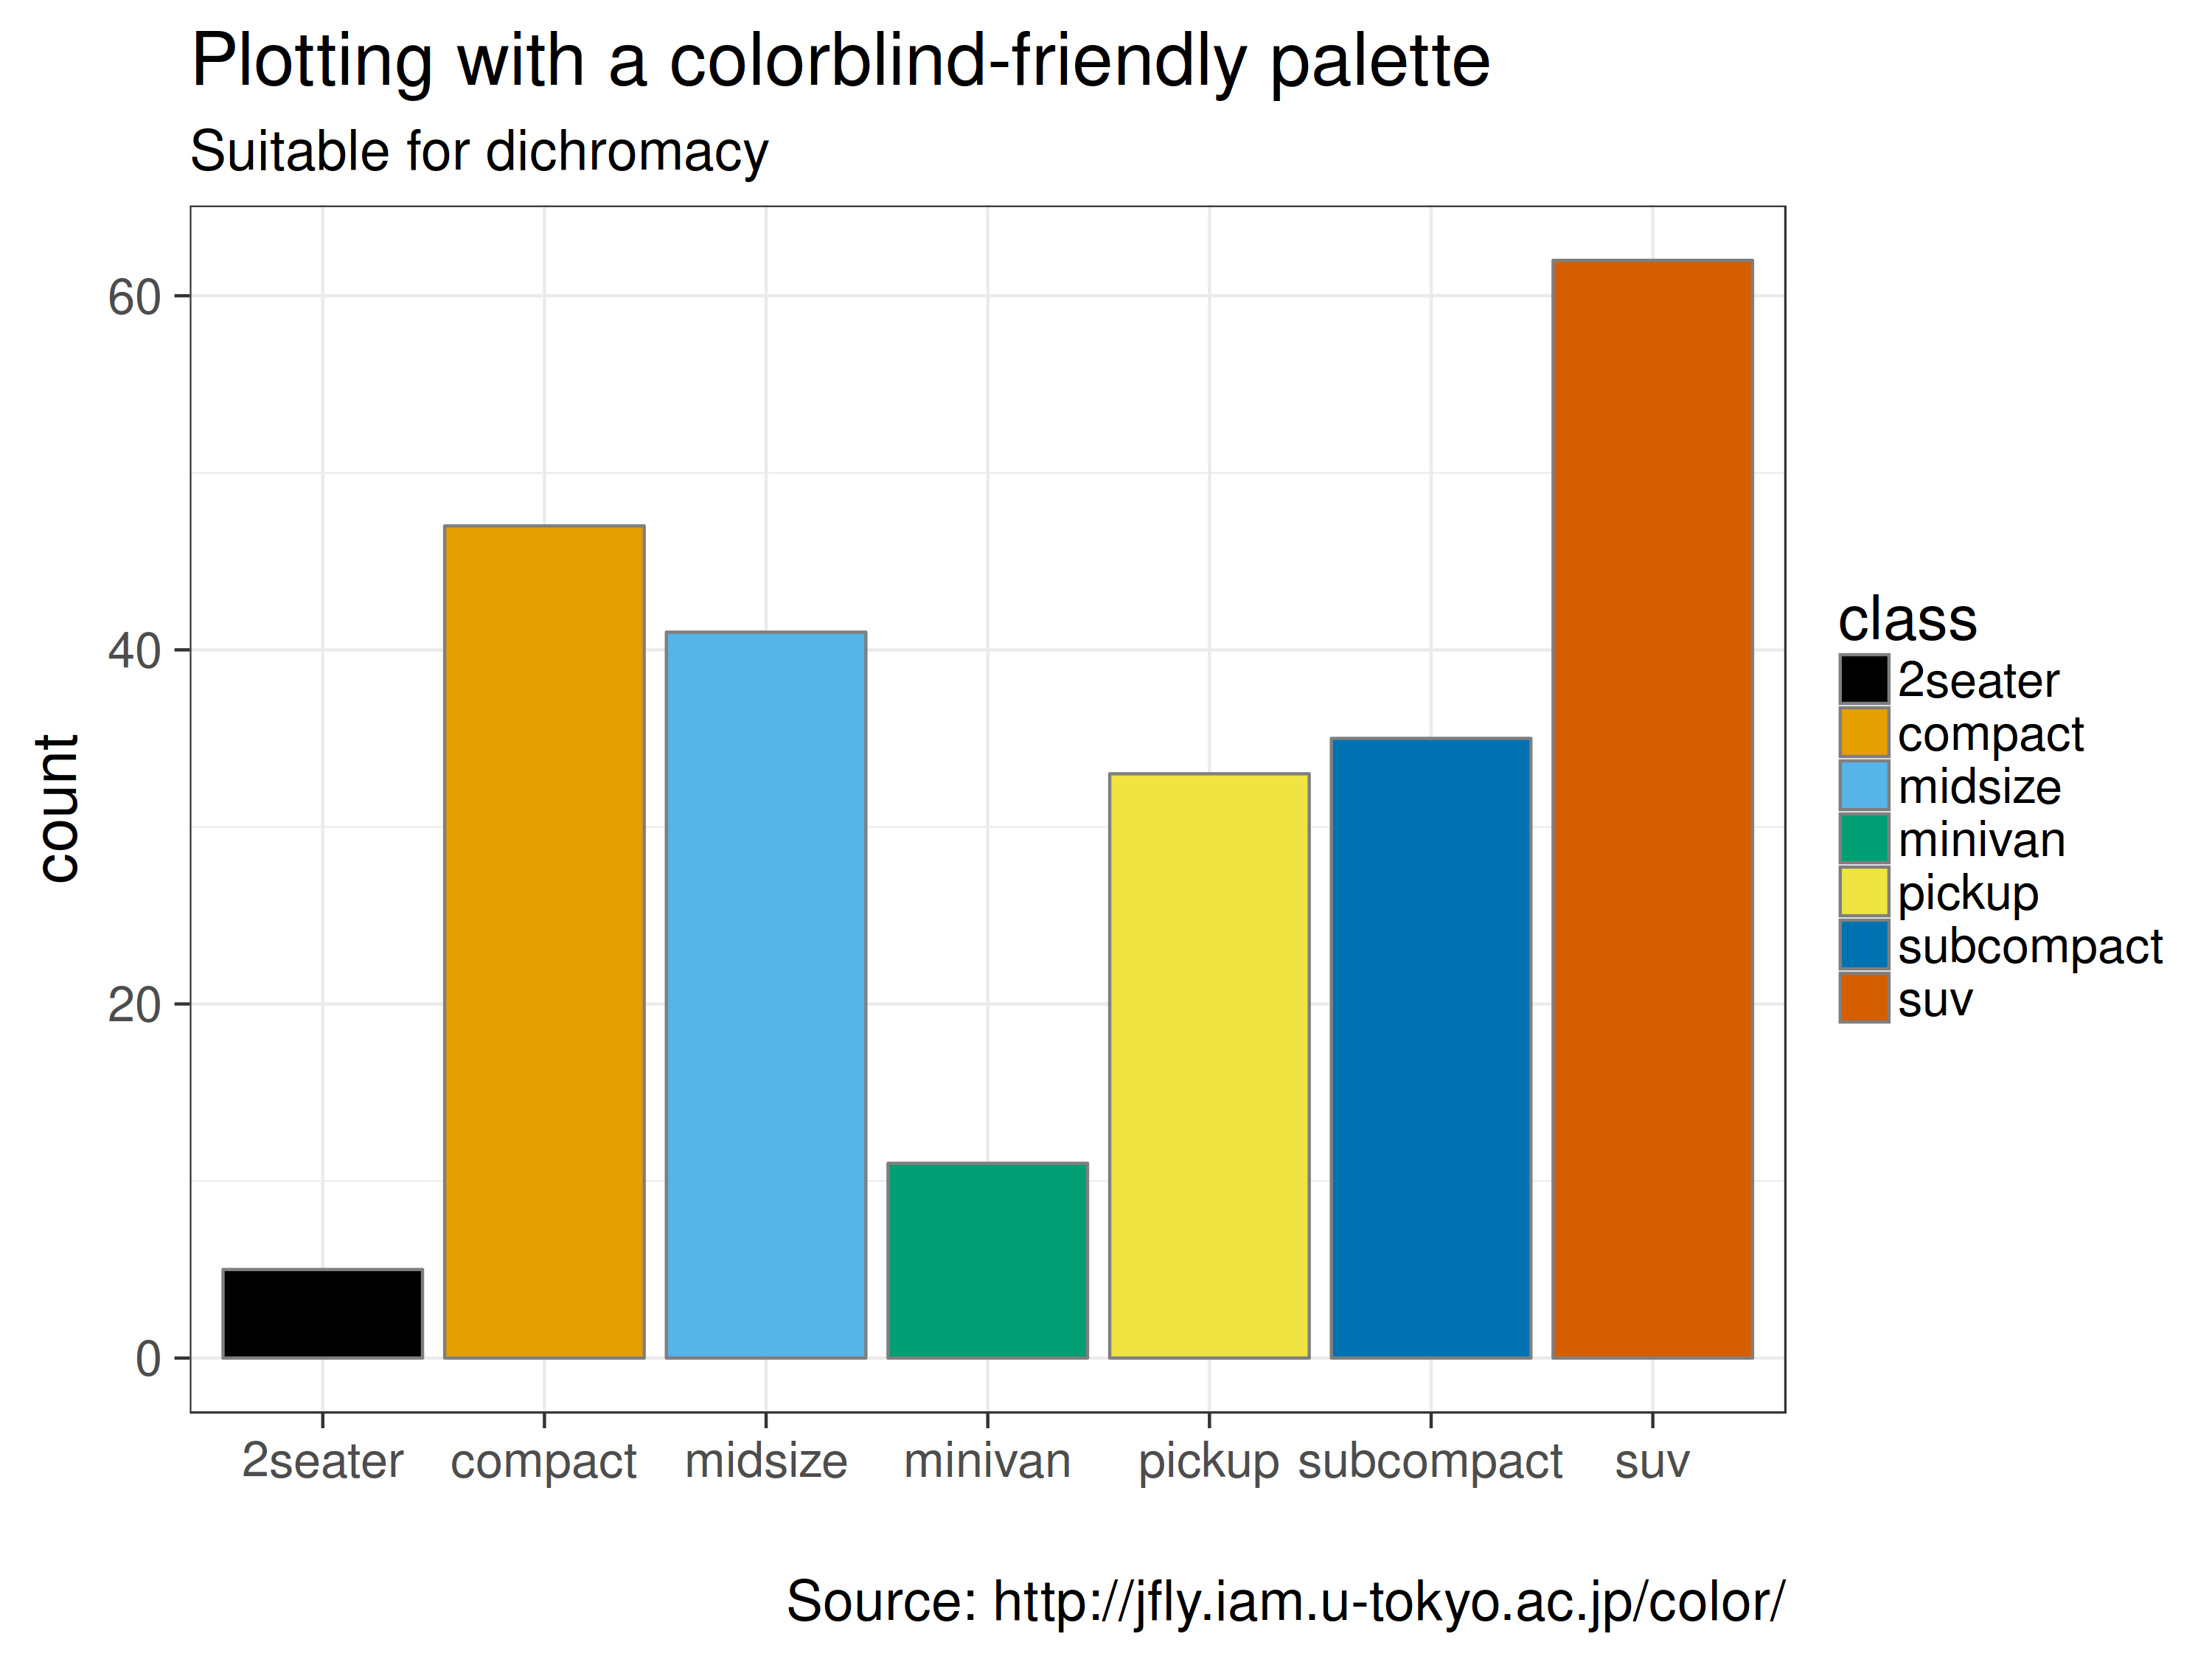
\includegraphics[width=0.9\linewidth]{figures/barchart-defaultfont.png}
    \caption{My figure}
  \end{figure}

  \small The default ggplot2 typeface is Helvetica
  
\end{frame}

% -----------------------------------------------------------------------

\begin{frame}
  \begin{figure}[htp!]
    \centering
    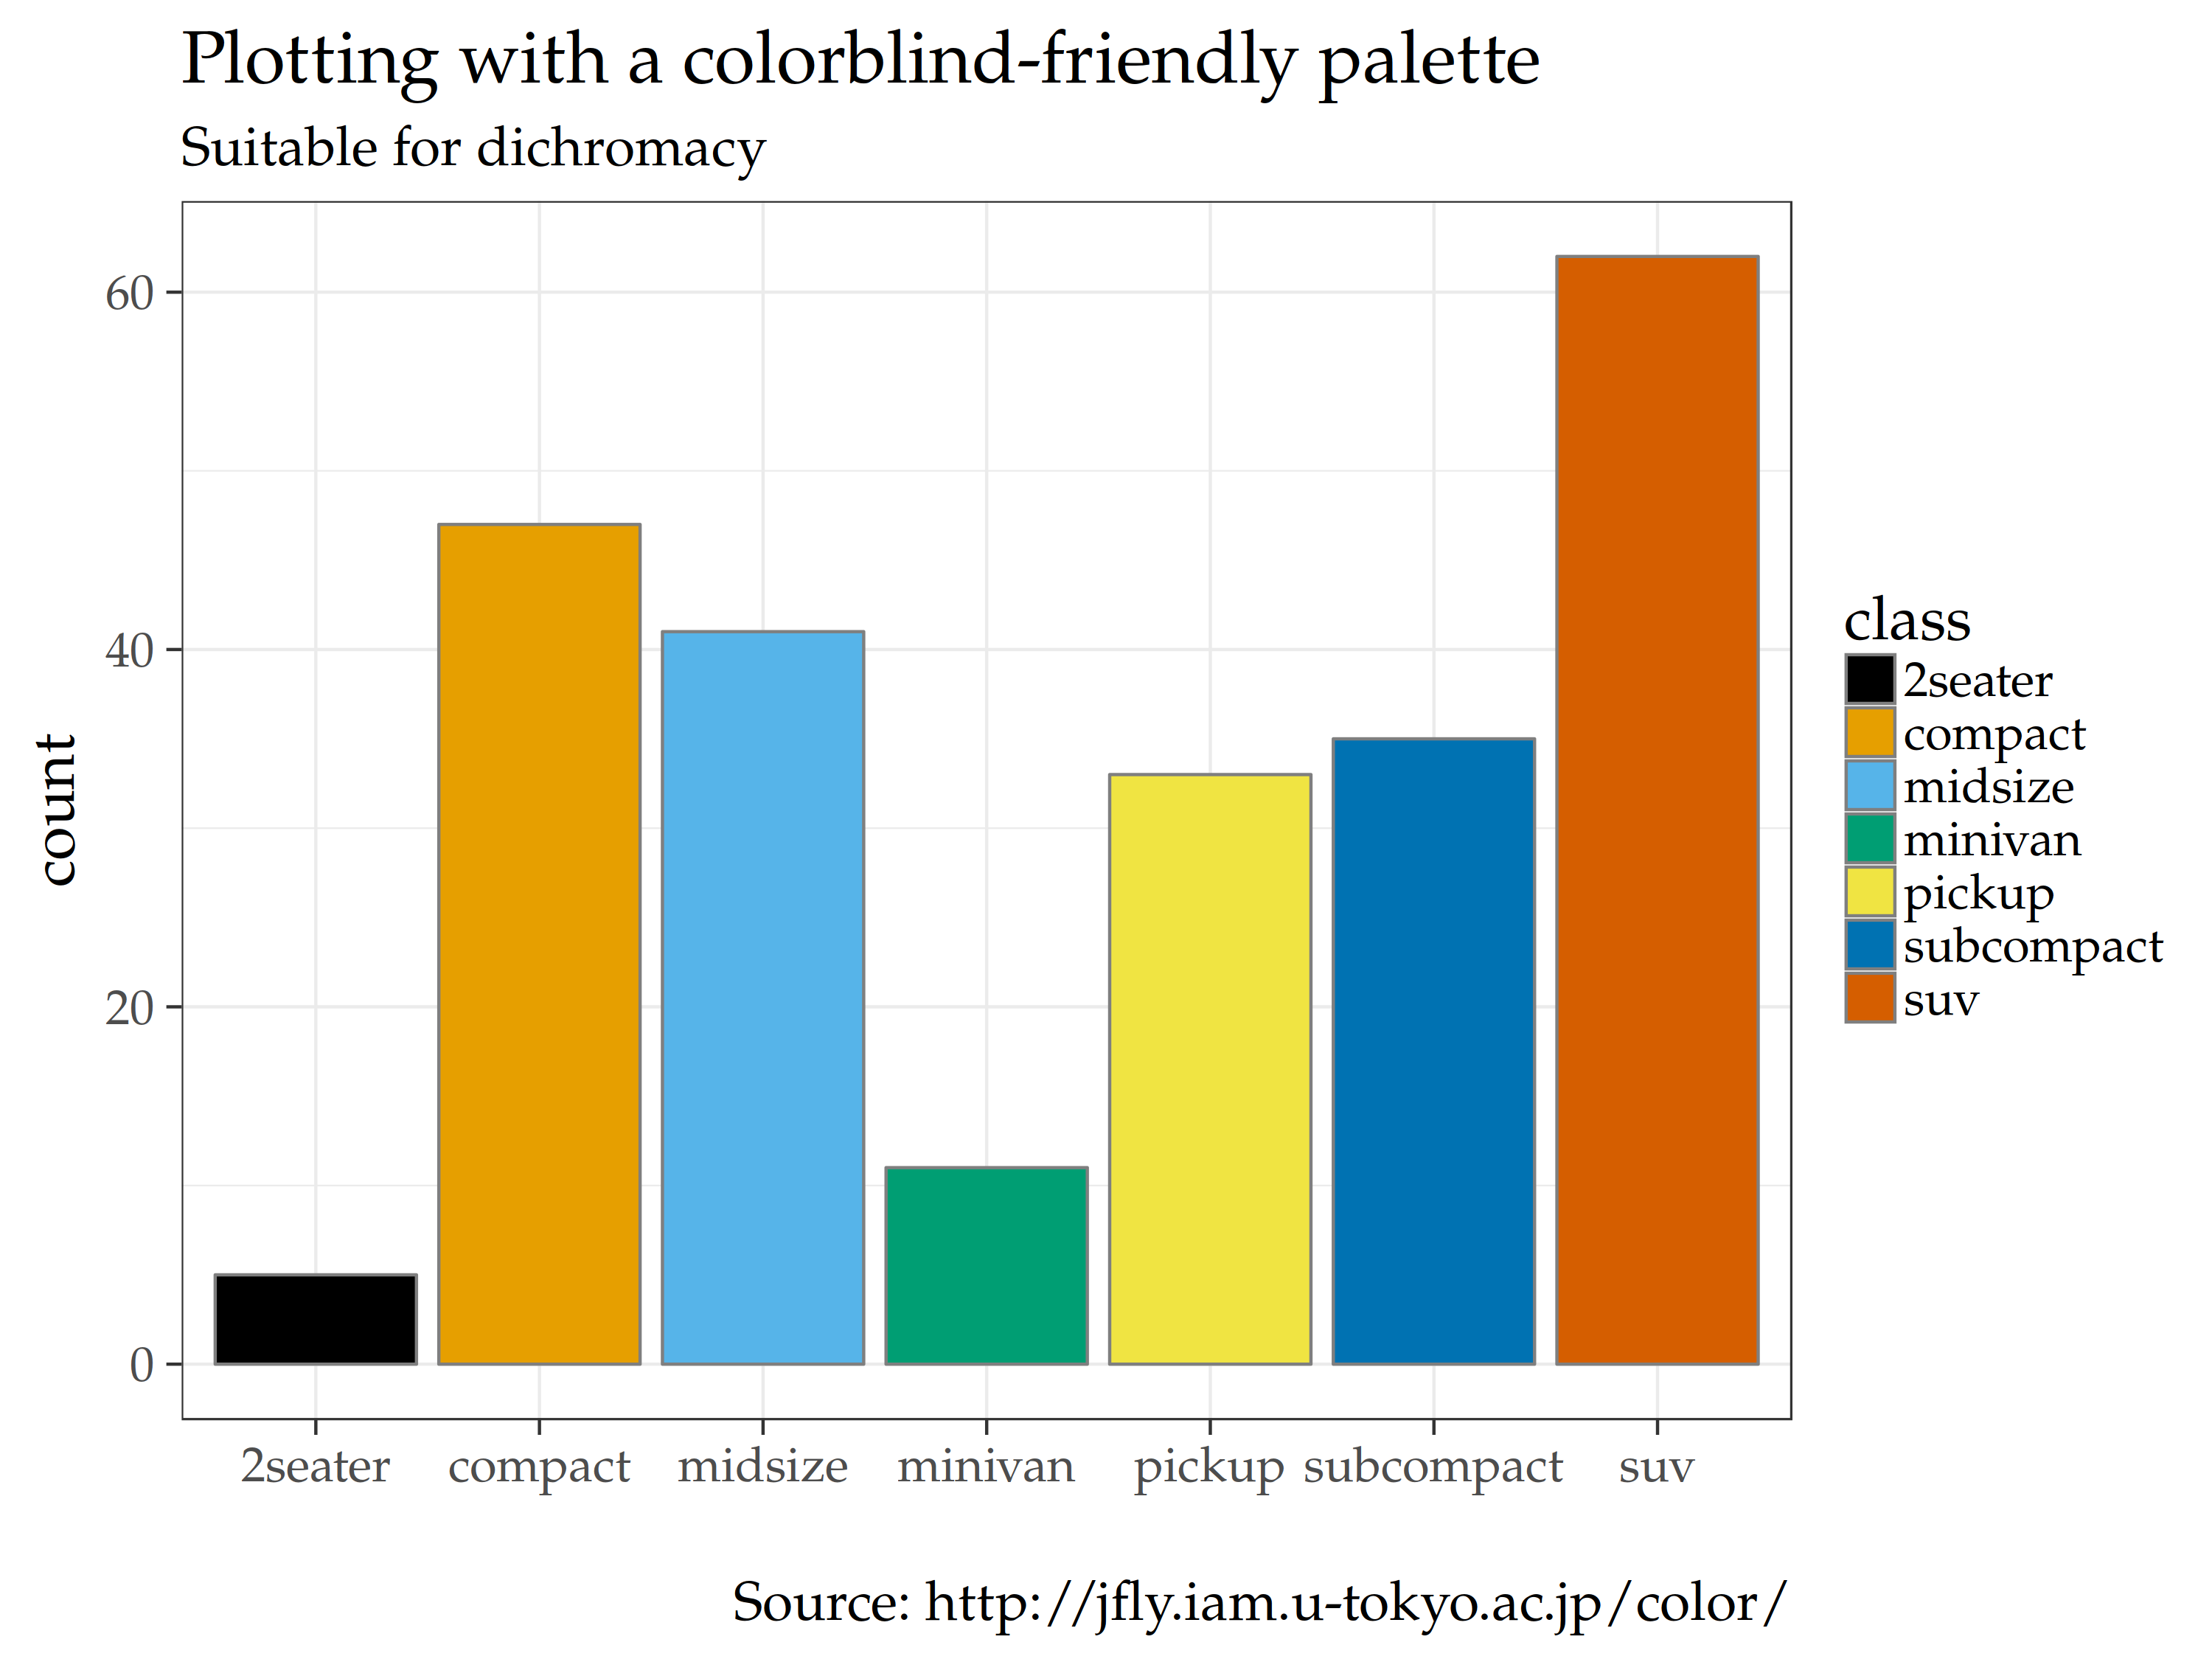
\includegraphics[width=0.9\linewidth]{figures/barchart-palatino.png}
  \end{figure}
  
  \small Palatino 
  
\end{frame}

% -----------------------------------------------------------------------

\begin{frame}
  \begin{figure}[htp!]
    \centering
    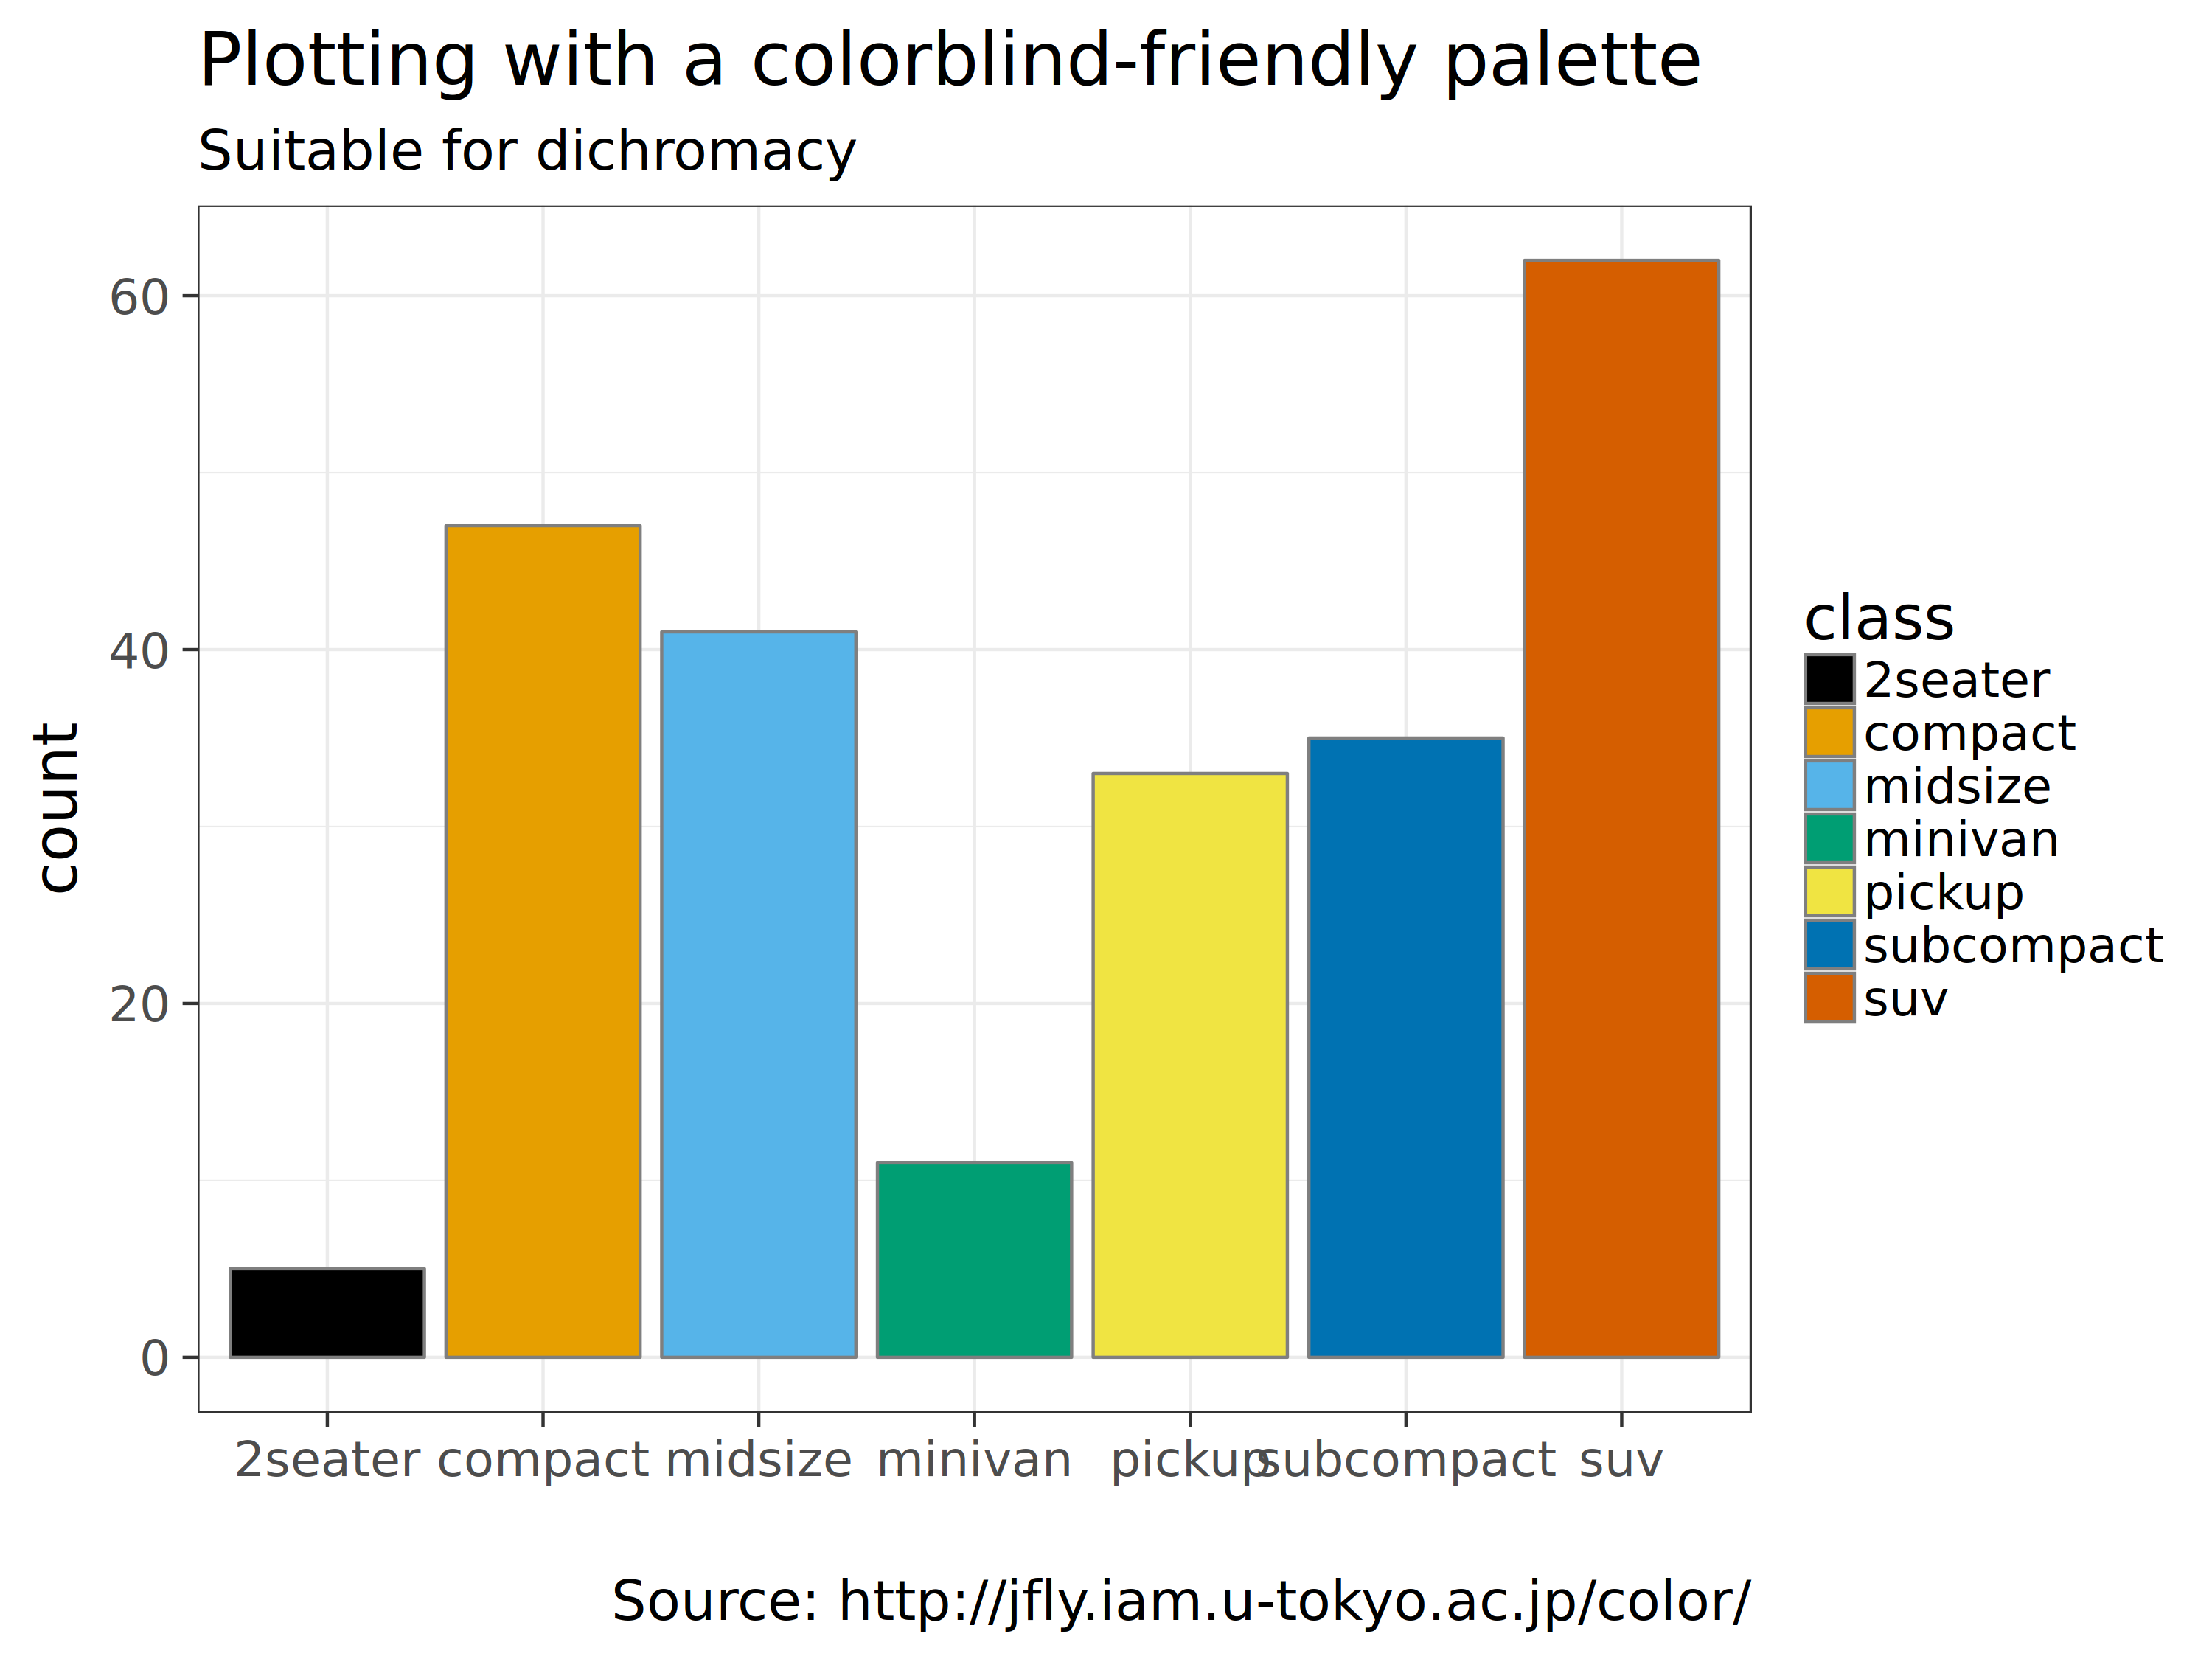
\includegraphics[width=0.9\linewidth]{figures/barchart-latosans.png}
  \end{figure}

  \small Lato Sans 
  
\end{frame}

% -----------------------------------------------------------------------

\begin{frame}
  \begin{figure}[htp!]
    \centering
    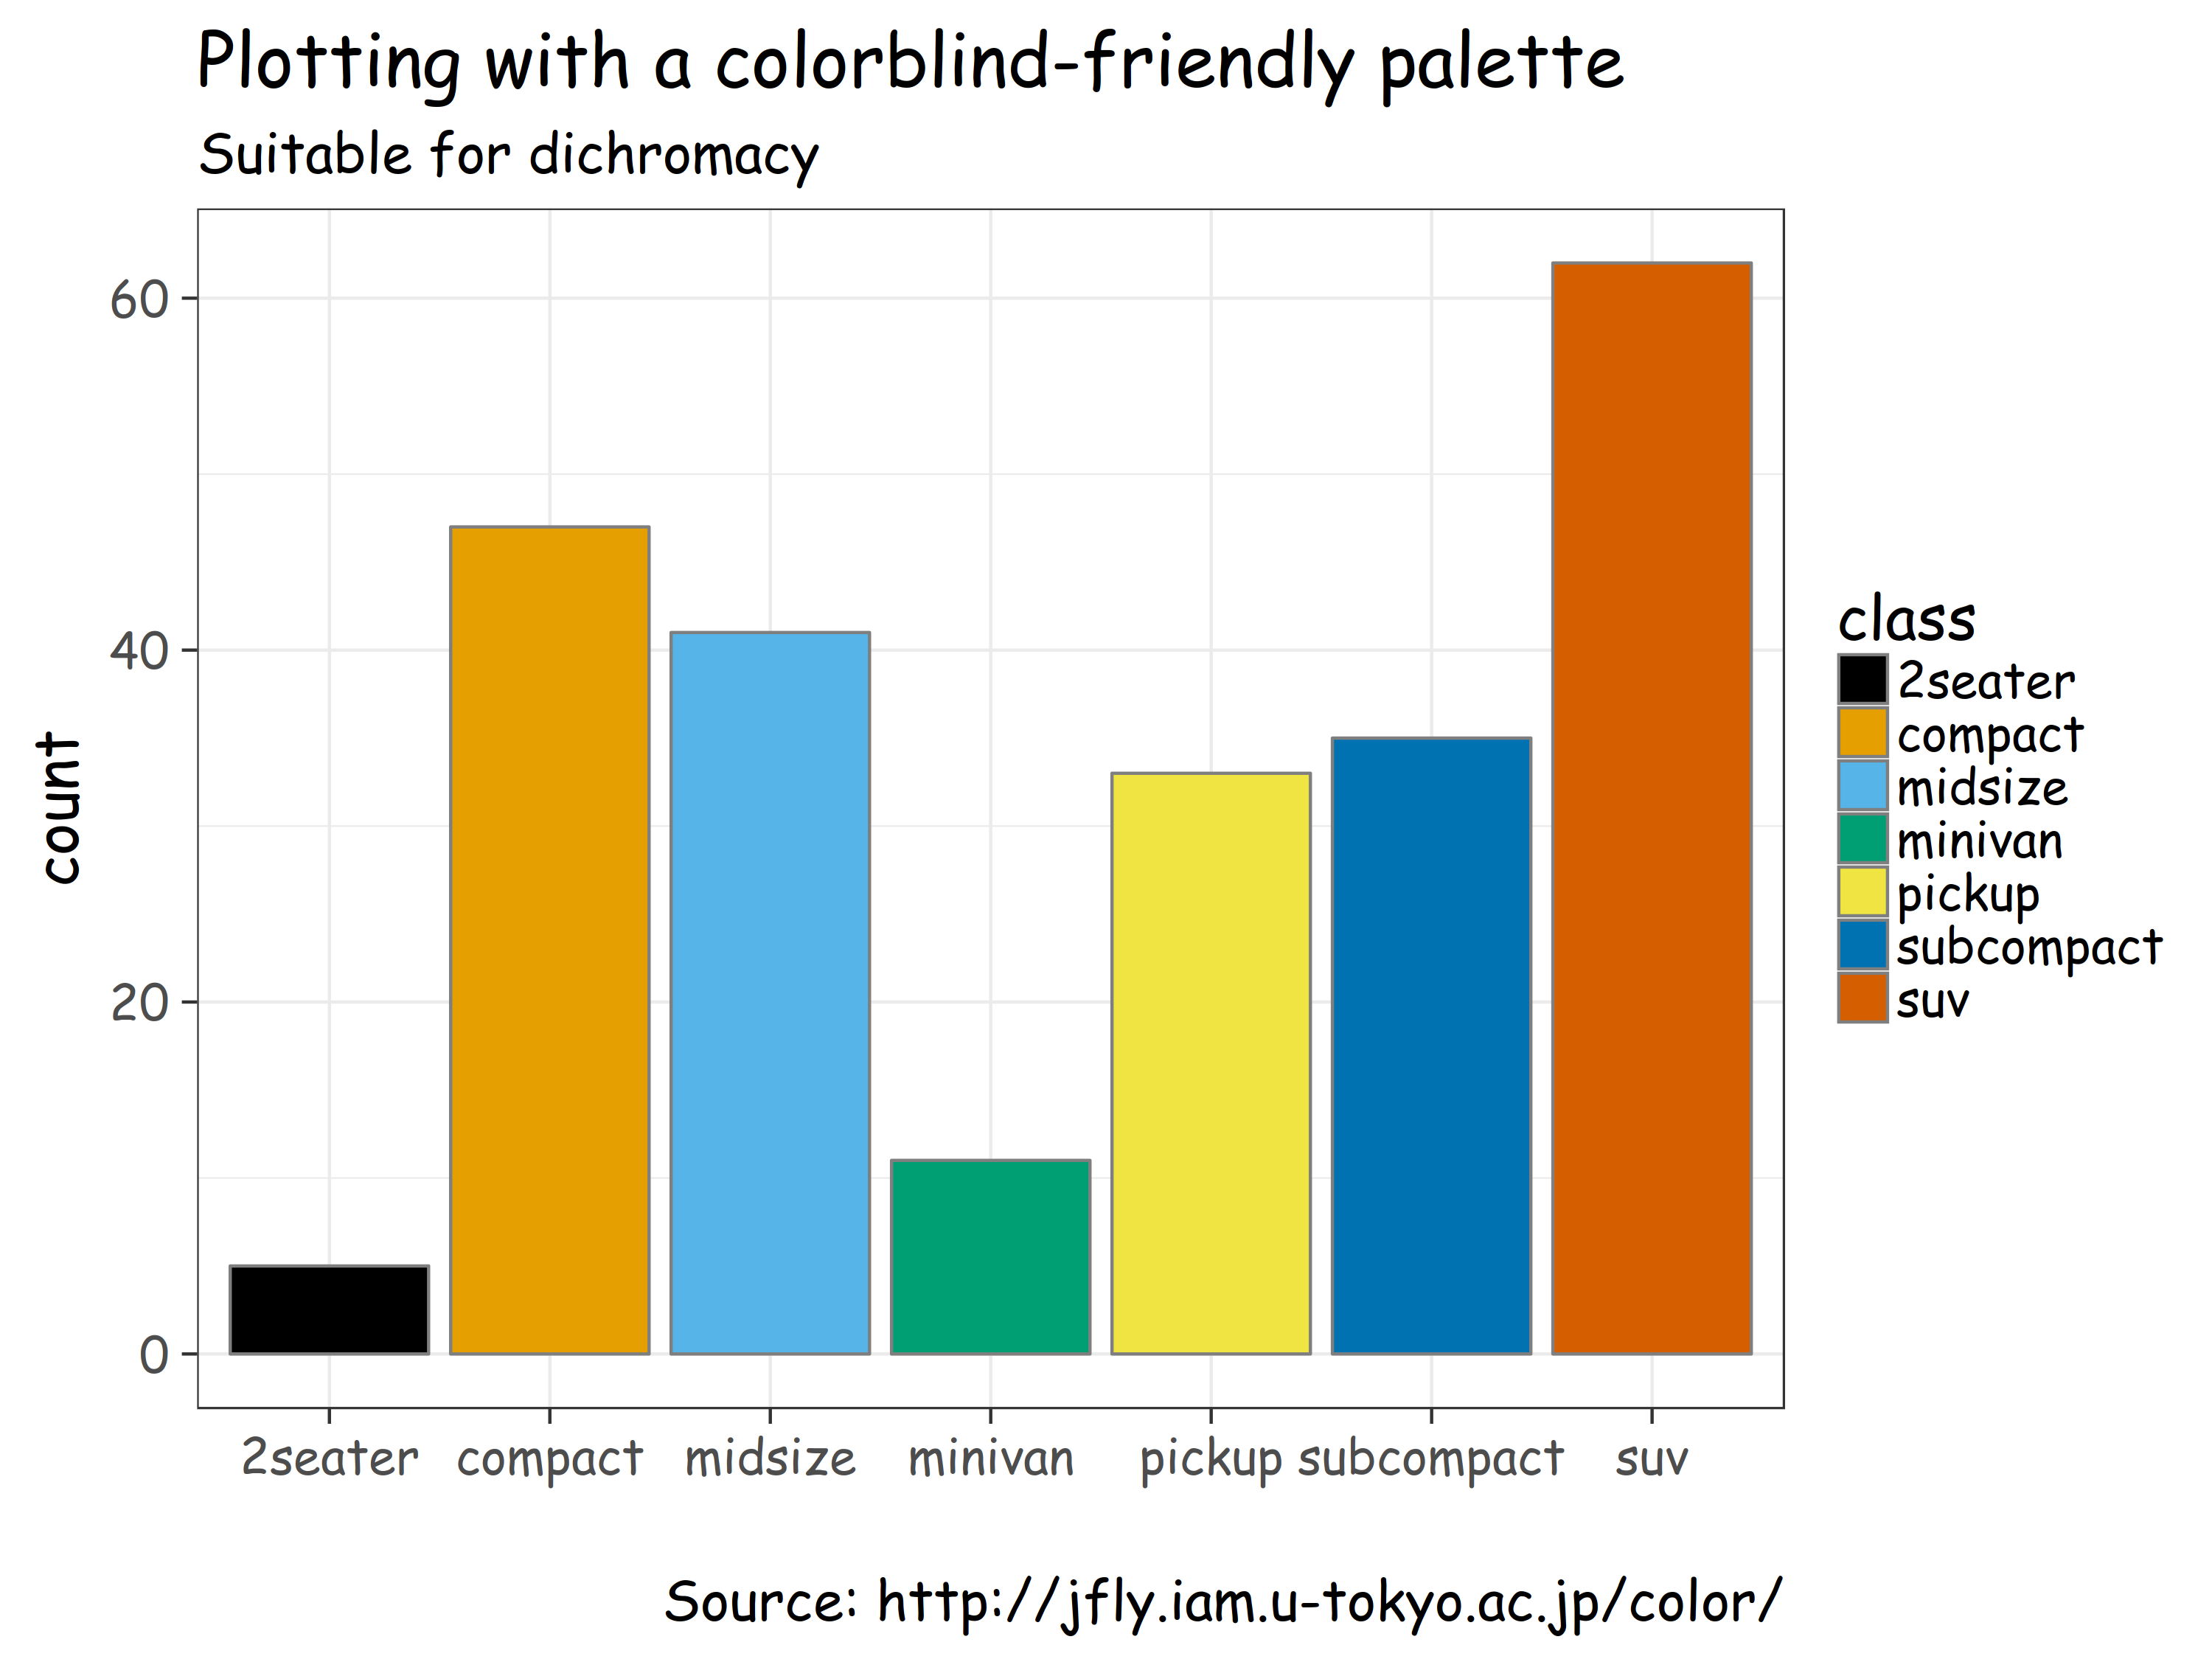
\includegraphics[width=0.9\linewidth]{figures/barchart-comicsansms.png}
  \end{figure}

  \small Comic Sans
\end{frame}

% -----------------------------------------------------------------------

%%% Local Variables:
%%% mode: latex
%%% TeX-master: "../main"
%%% End:
